\section{Context}
\label{sec:context}

De gebruikers van het systeem zijn onder te verdelen in 5 categorie\"{e}n: externen, studenten, professoren, assistenten en programmabeheerders. 
Het design van CalZone houdt rekening met de functionaliteiten die specifiek aan deze gebruikers zijn toegekend zoals beschreven in het SRS\cite{SRS} van dit project. 
\\

De functionaliteiten die iedere actor in het systeem bezit, worden ge\"{i}llustreerd in de use case diagrammen  \ref{fig:useCaseUsers}, \ref{fig:useCaseAdmin}, \ref{fig:useCaseProf} en \ref{fig:useCaseStudent}.

\begin{figure}[H]
	\centering
	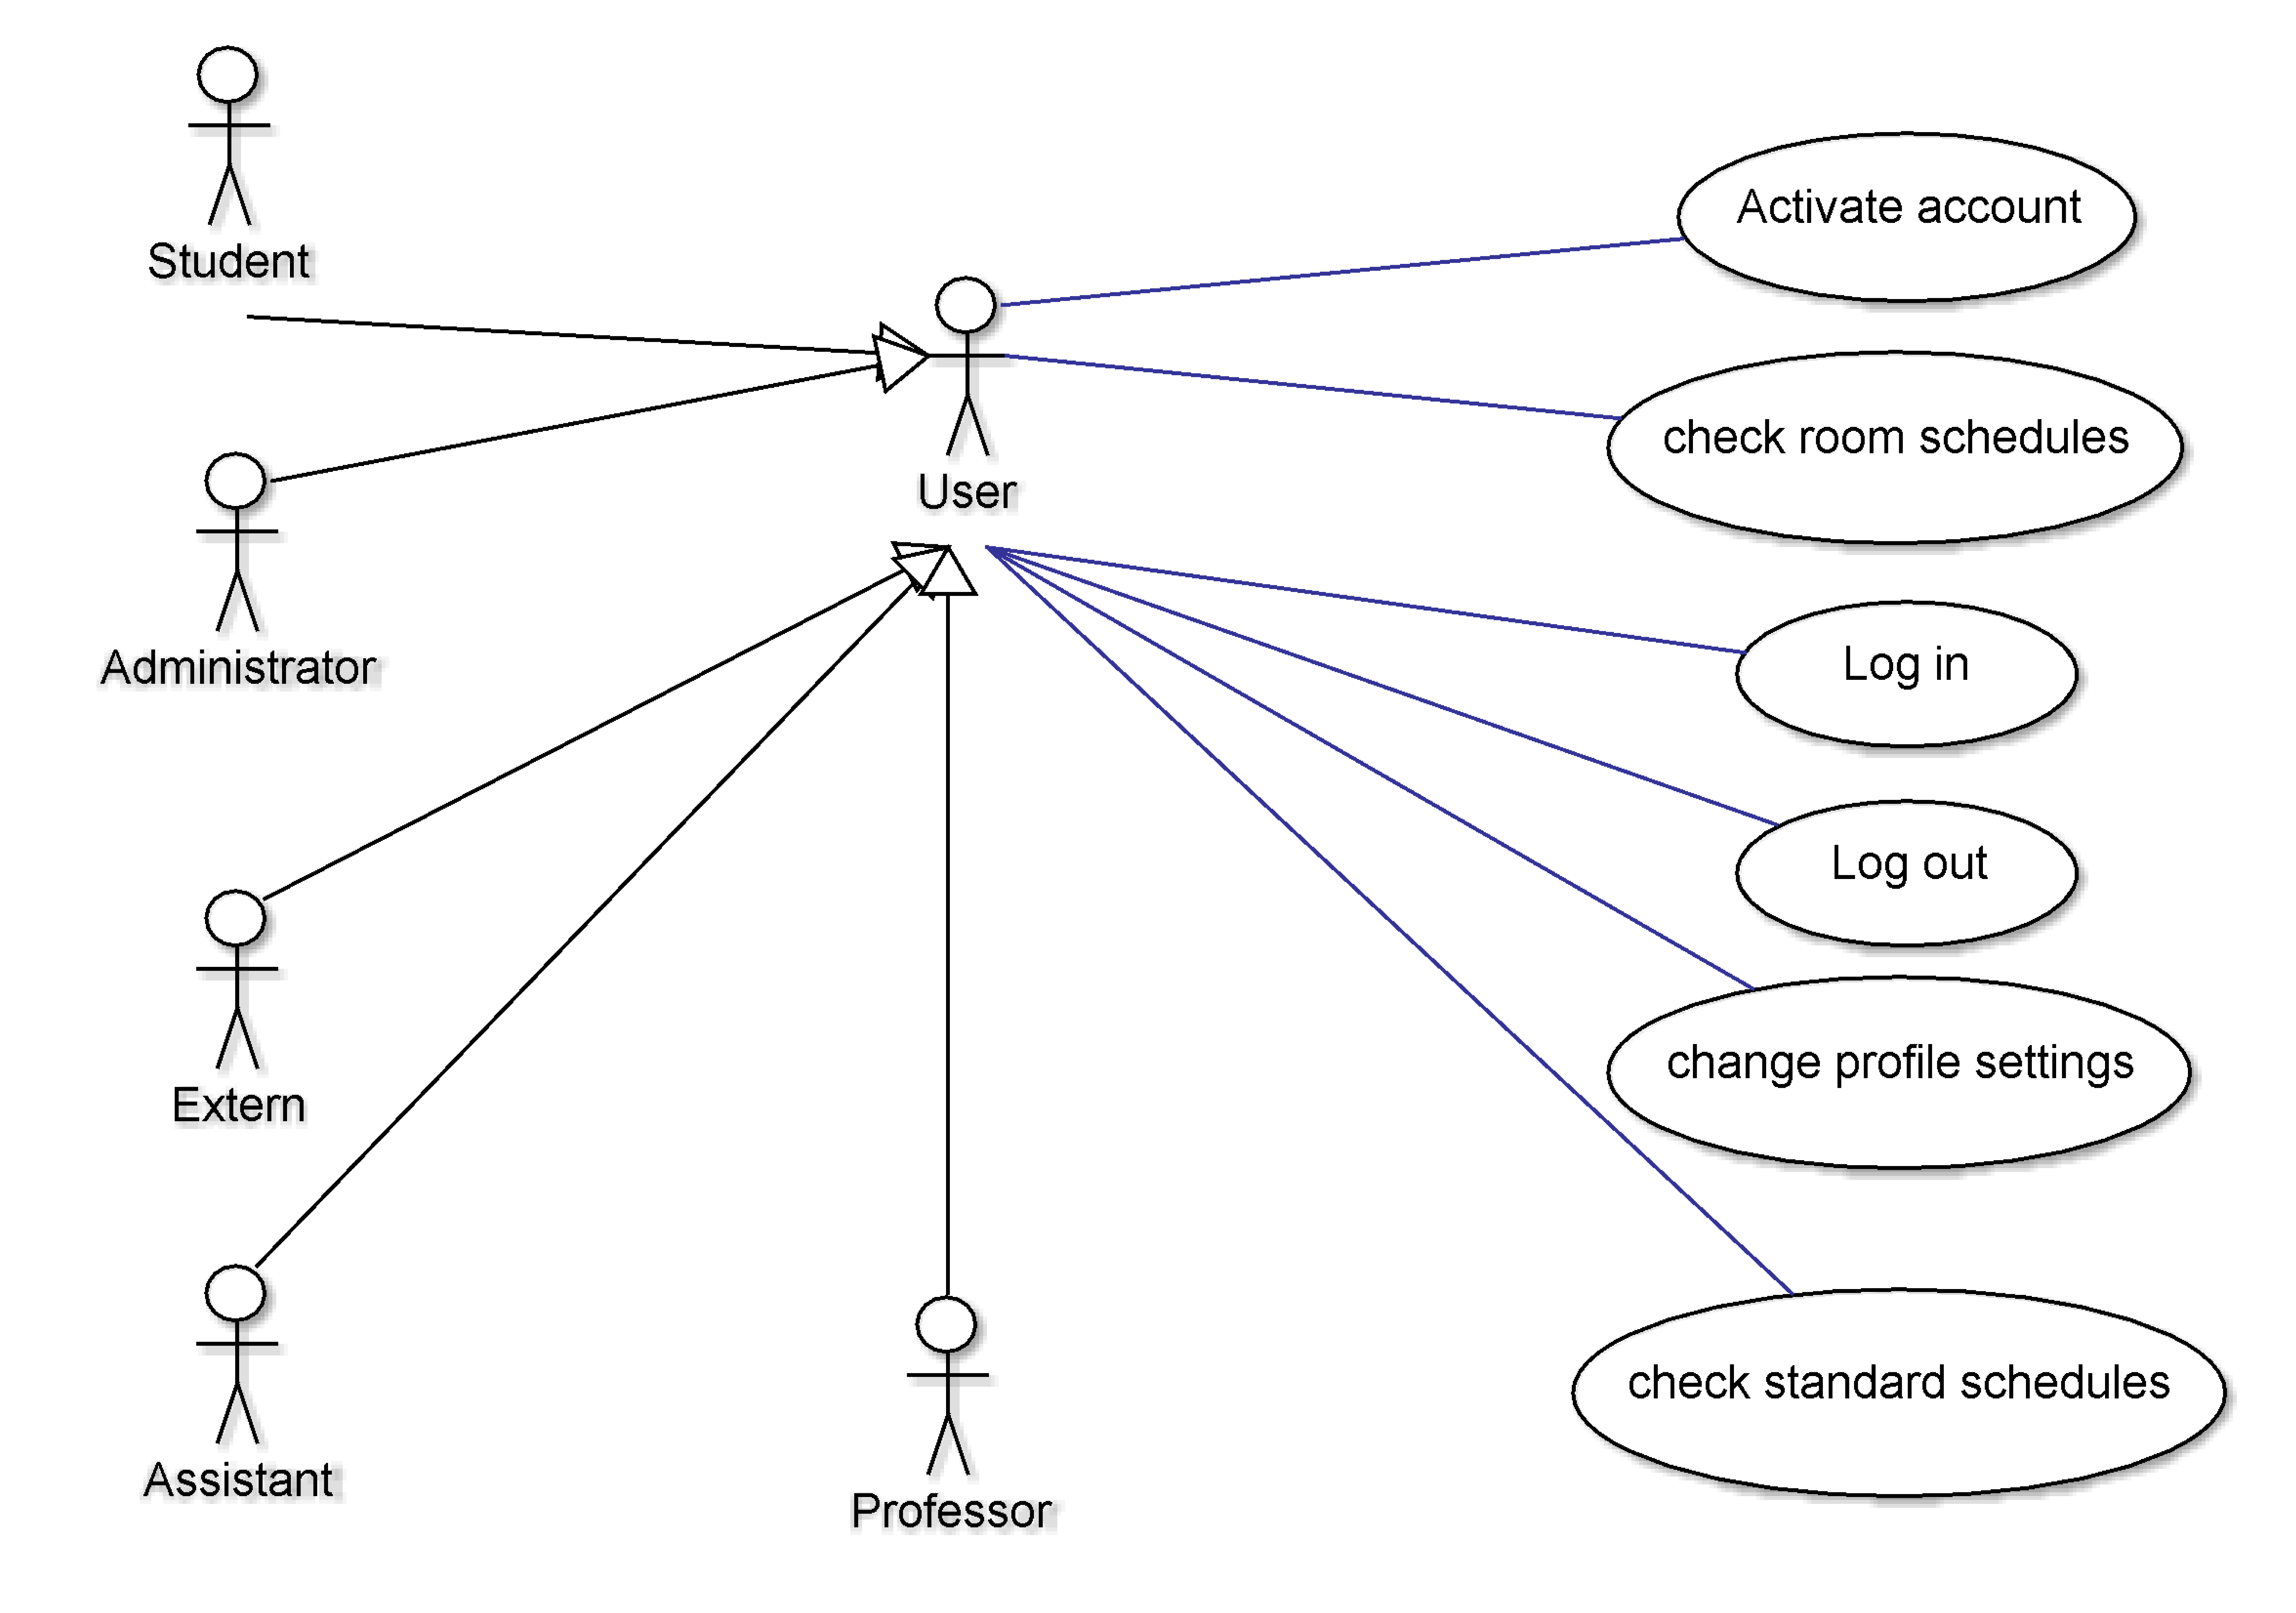
\includegraphics[scale=0.2]{img/useCaseUsers}
	\caption{Use case diagram met focus op de verschillende actoren}
	\label{fig:useCaseUsers}
\end{figure}

\begin{figure}[H]
	\centering
	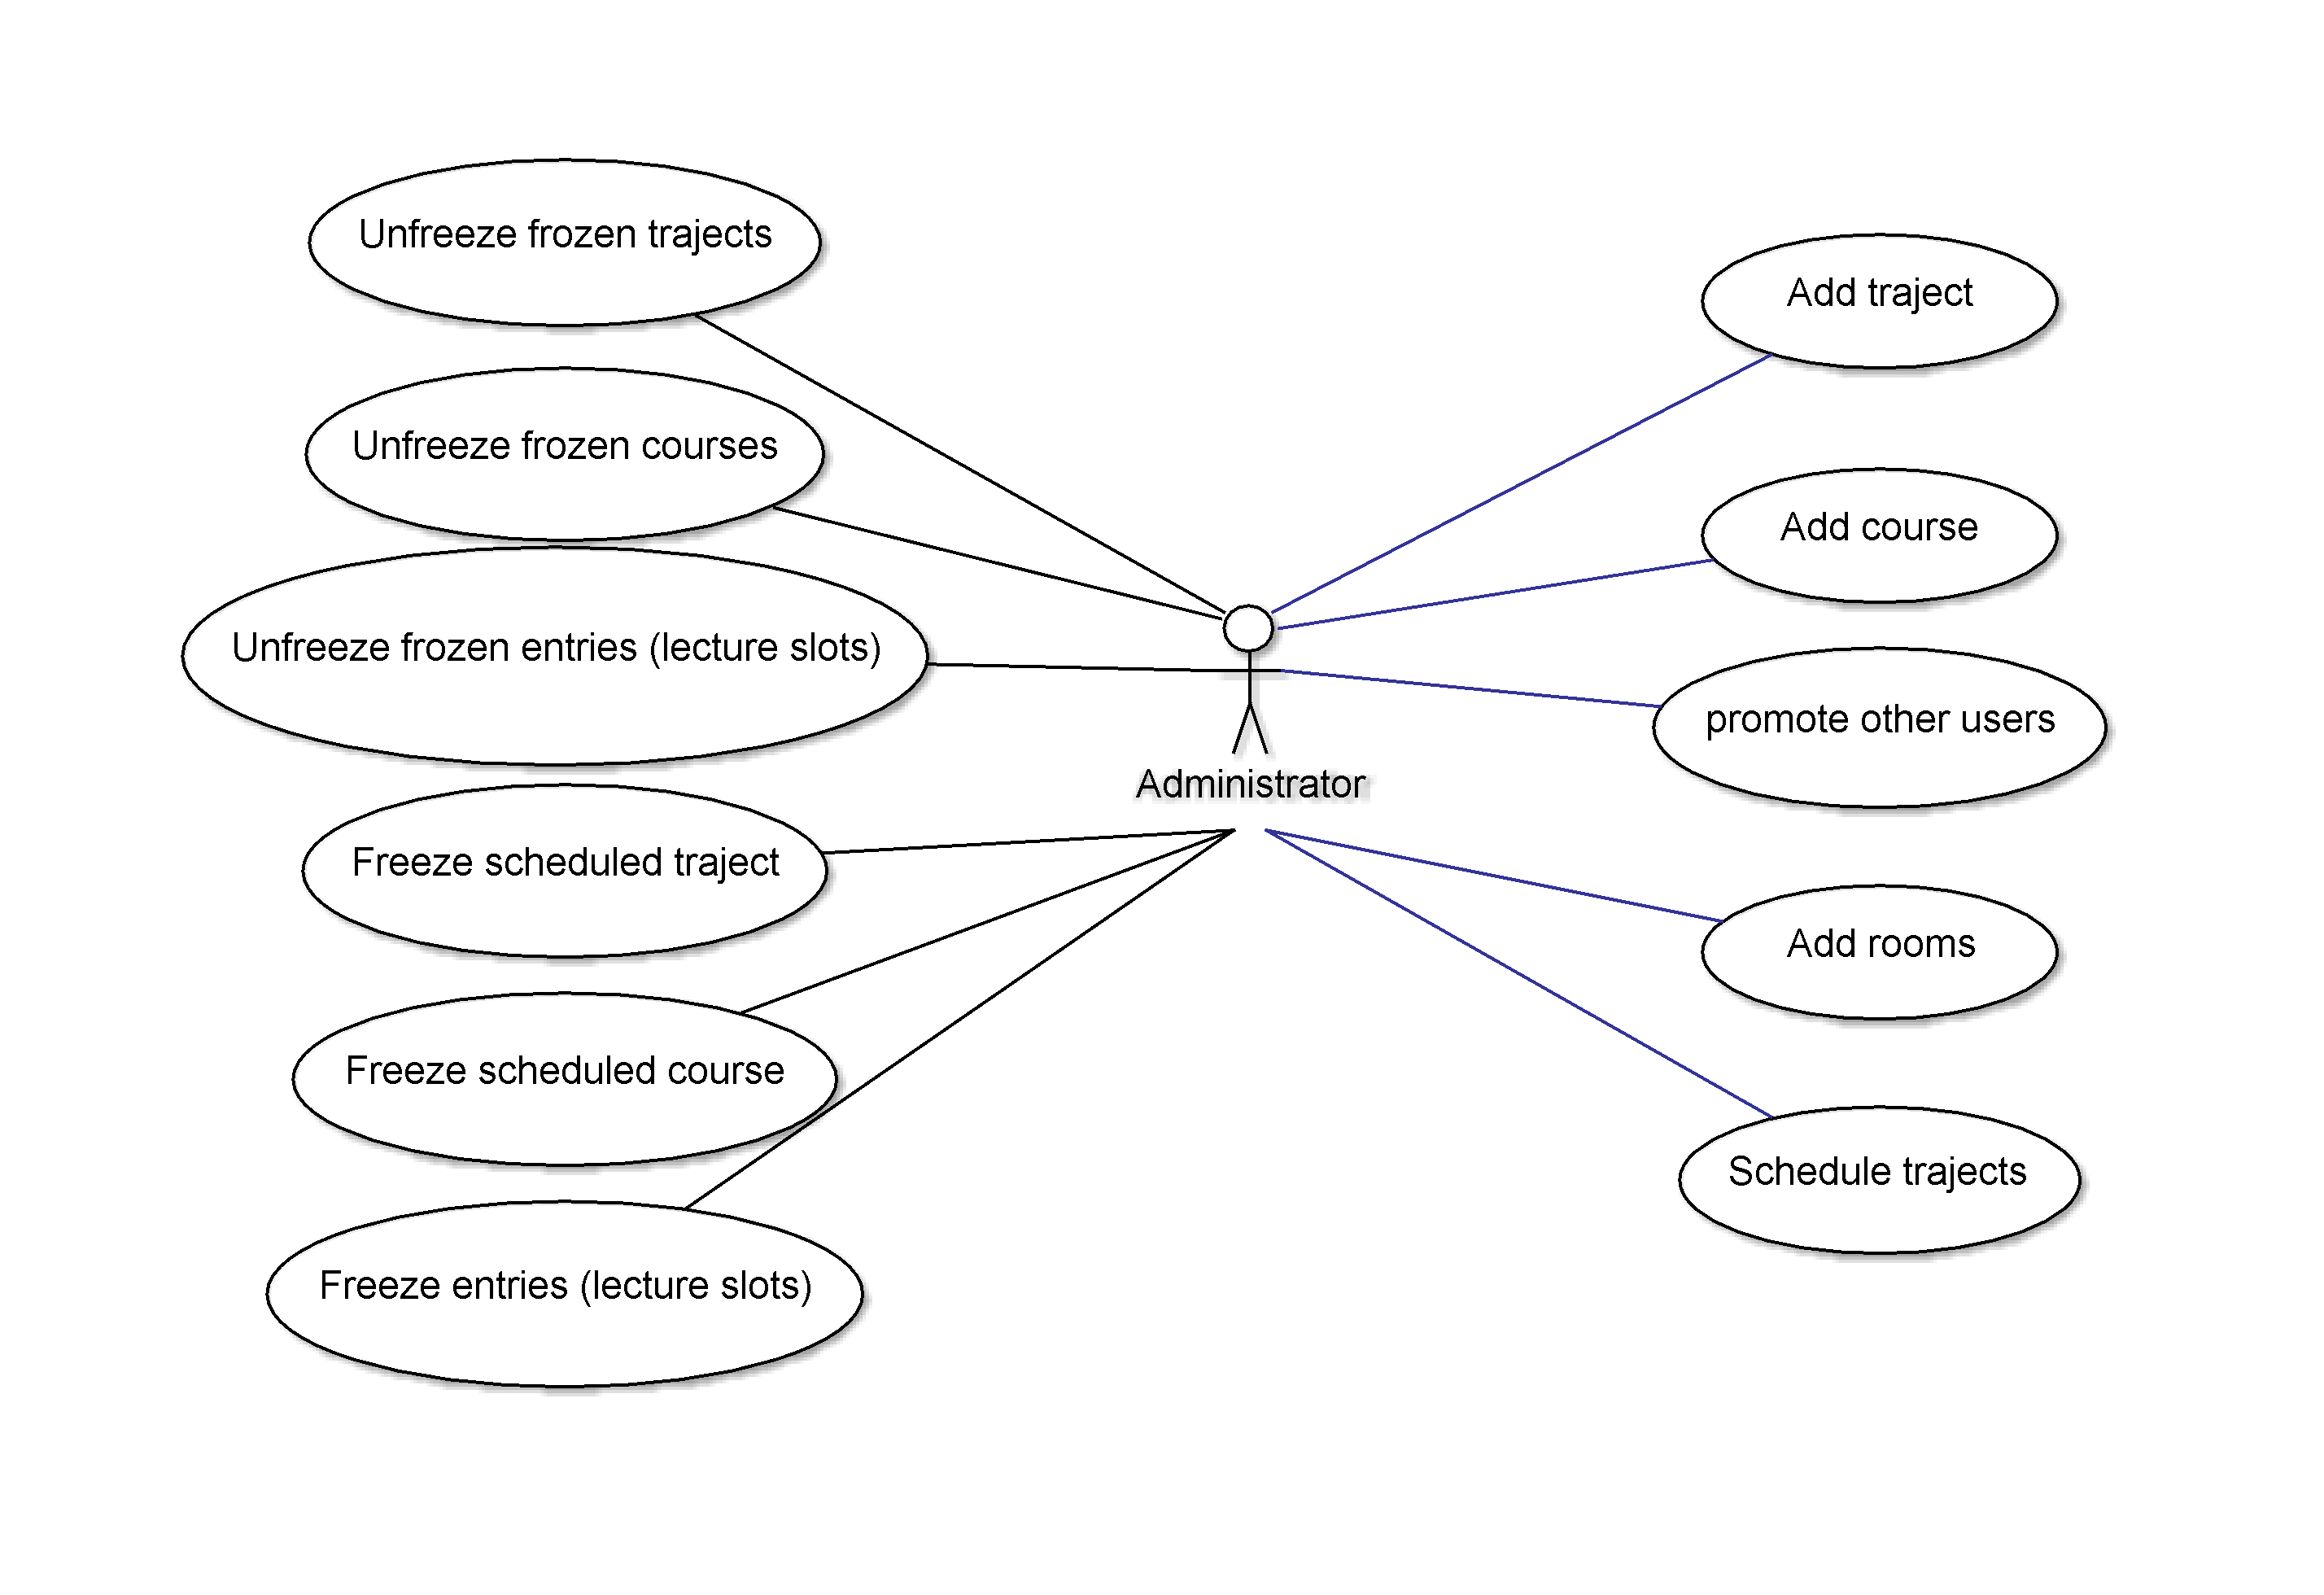
\includegraphics[scale=0.15]{img/useCaseAdmin}
	\caption{Use case diagram met focus op de actor administrator}
	\label{fig:useCaseAdmin}
\end{figure}

\begin{figure}[H]
	\centering
	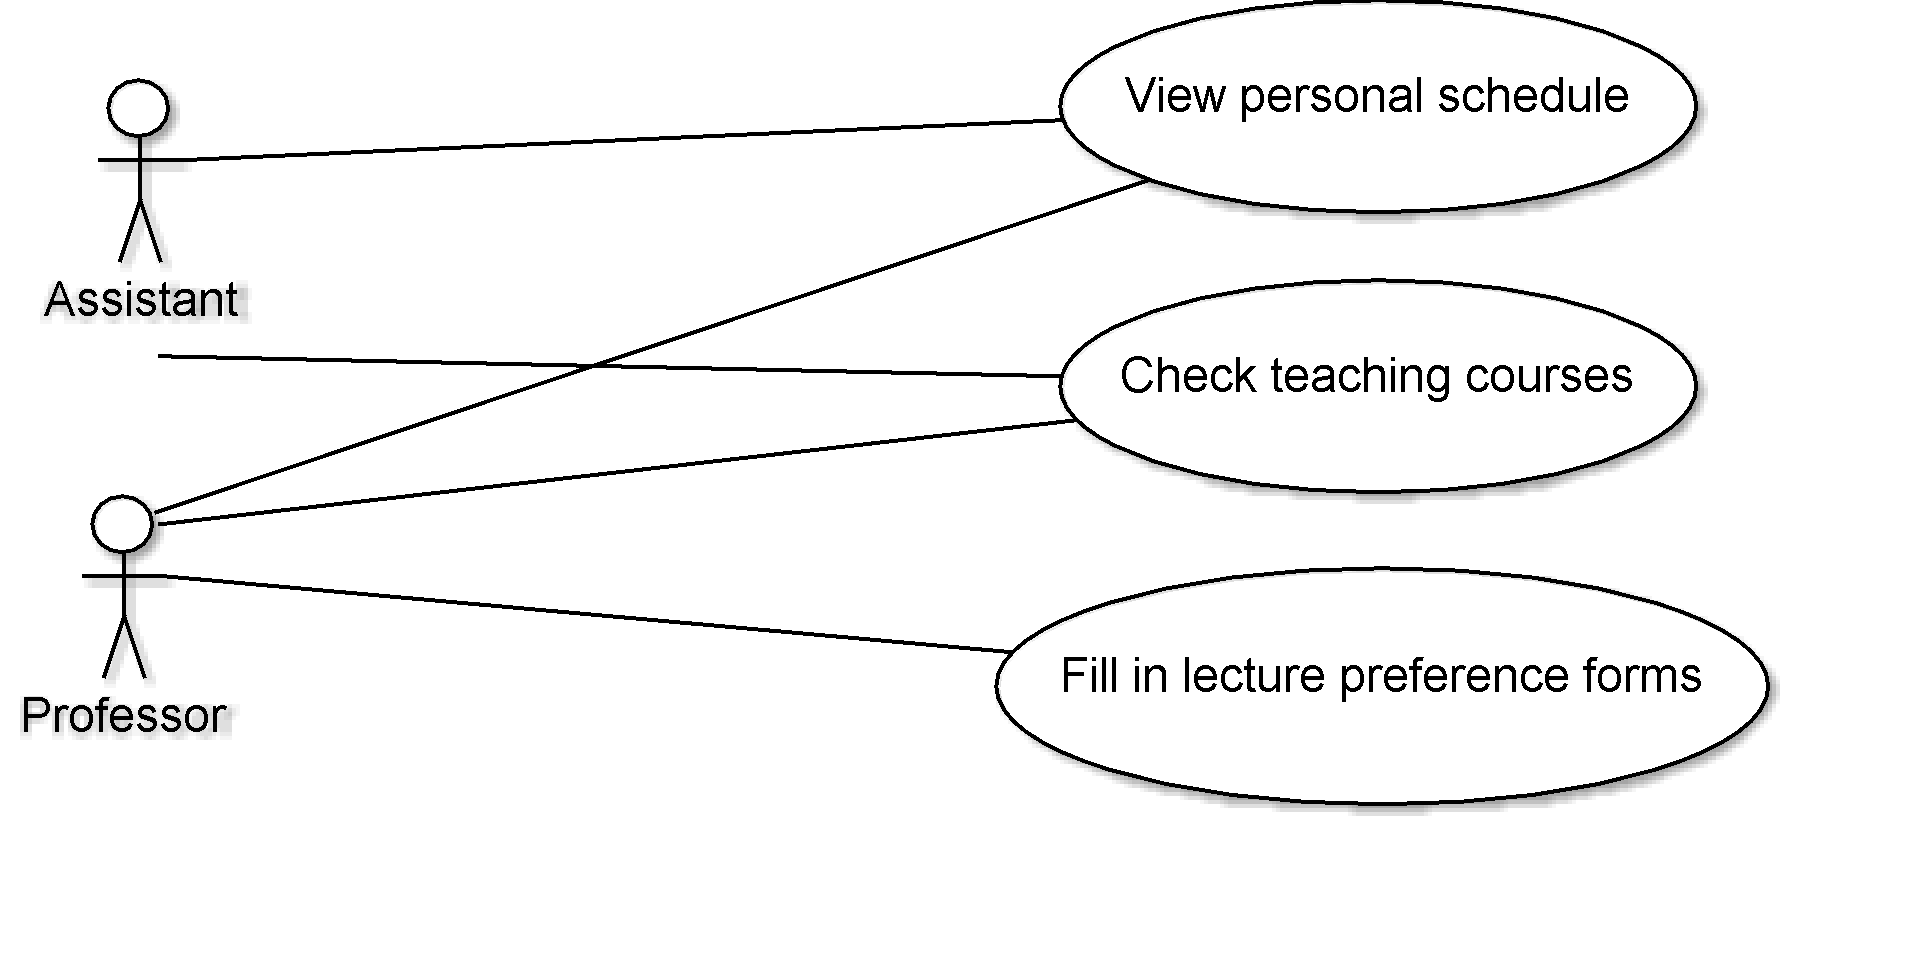
\includegraphics[scale=0.2]{img/useCaseProf}
	\caption{Use case diagram met focus op de actoren professor en assistant}
	\label{fig:useCaseProf}
\end{figure}

\begin{figure}[H]
	\centering
	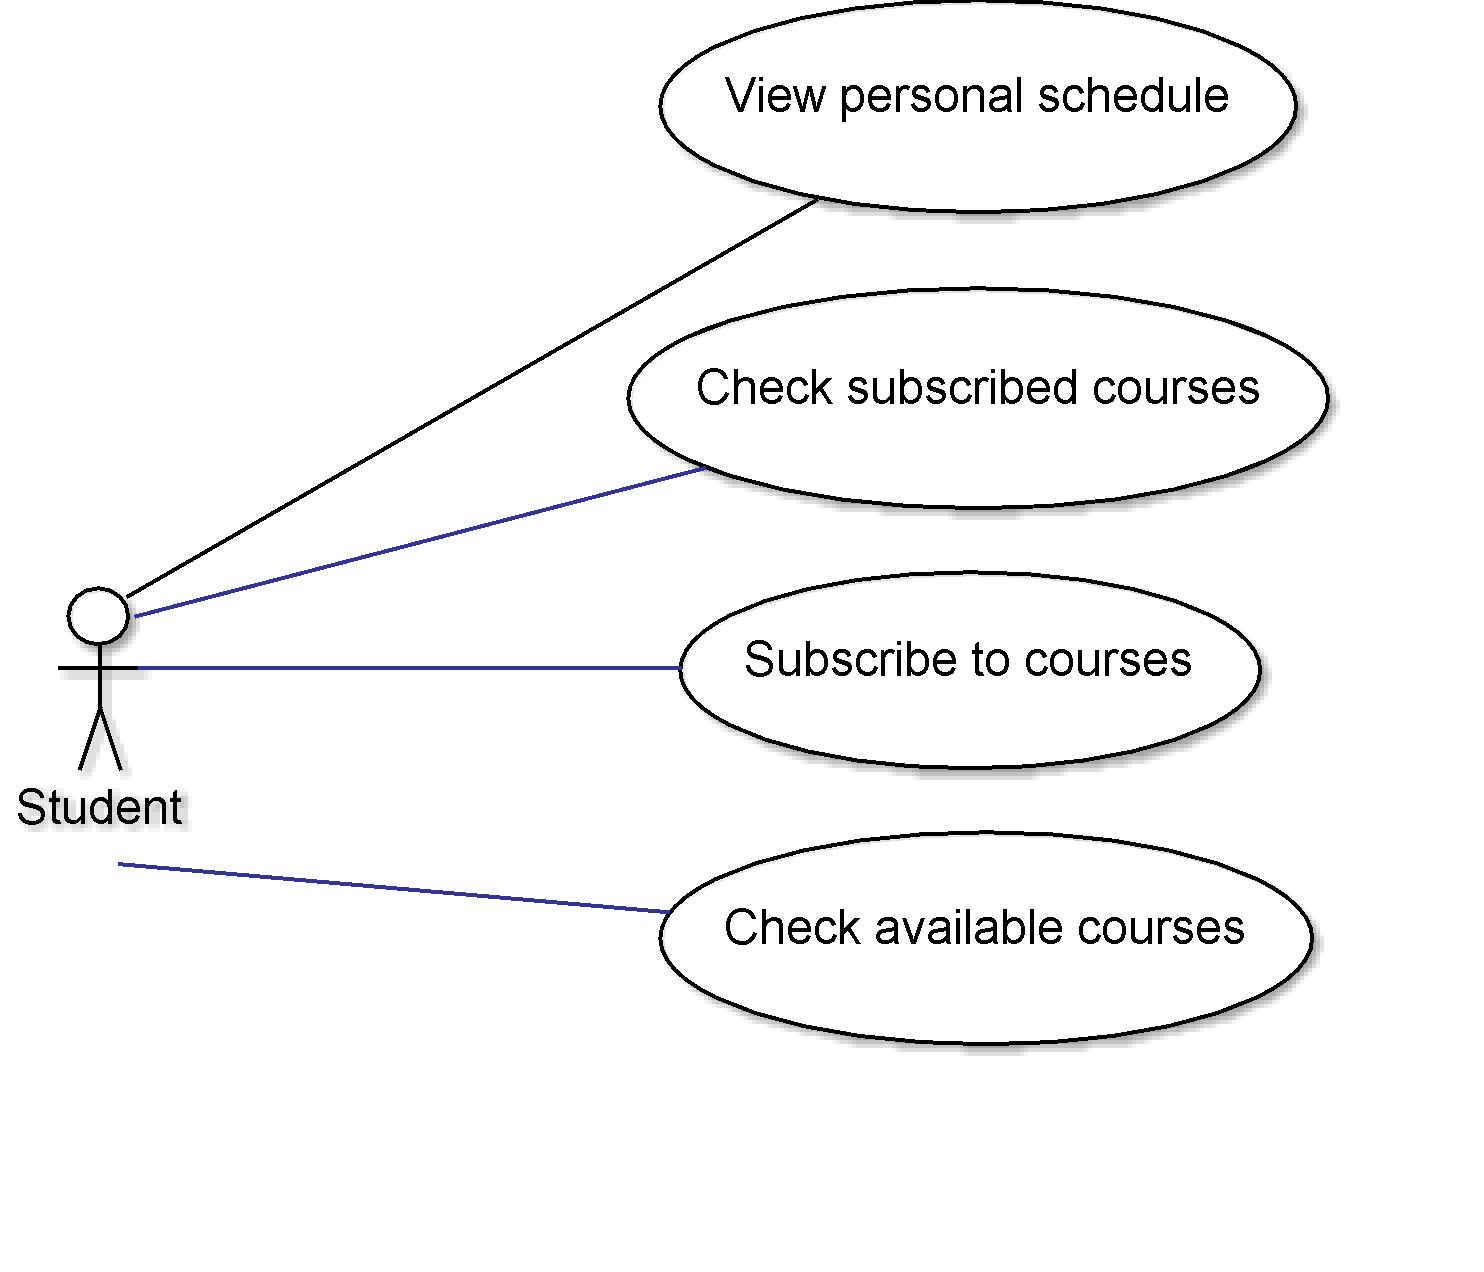
\includegraphics[scale=0.2]{img/useCaseStudent}
	\caption{Use case diagram met focus op de actor student}
	\label{fig:useCaseStudent}
\end{figure}